% Auto-generated from practice_sheet.tex
\documentclass[10pt]{article}
\usepackage[legalpaper,margin=0.5in]{geometry}
\usepackage[T1]{fontenc}
\usepackage[utf8]{inputenc}
\usepackage{FiraSans}
\usepackage[scaled=0.95]{FiraMono}
\usepackage{amsmath,amssymb,amsthm,mathtools}
\usepackage{booktabs,array,tabularx,multirow}
\usepackage{graphicx}
\usepackage{tikz}
\usepackage{pgfplots}
\usepackage{xcolor}
\usepackage{enumitem}
\usepackage{hyperref}
\usepackage{fancyhdr}
\usepackage{titlesec}
\usepackage[most]{tcolorbox}
\usetikzlibrary{arrows.meta,positioning,calc,patterns,decorations.pathreplacing,fit,backgrounds}
\pgfplotsset{compat=1.18}

% Slide-matched colors
\definecolor{PrimaryColor}{RGB}{33,52,72}
\definecolor{SecondaryColor}{RGB}{84,119,146}
\definecolor{AccentColor}{RGB}{100,156,165}
\definecolor{BackgroundColor}{RGB}{245,247,250}
\definecolor{TextColor}{RGB}{40,55,70}
\definecolor{LightGray}{RGB}{220,225,230}
\definecolor{DarkGray}{RGB}{70,90,105}

\hypersetup{colorlinks=true,linkcolor=PrimaryColor,urlcolor=PrimaryColor}
\setlength{\parindent}{0pt}
\setlength{\parskip}{0.42em}
\setlength{\headheight}{14pt}
\renewcommand{\familydefault}{\sfdefault}
\renewcommand{\seriesdefault}{l}
\color{TextColor}

\pagestyle{fancy}
\fancyhf{}
\fancyhead[L]{CSE 219 Practice Questions}
\fancyhead[R]{FFT, Sampling, Laplace, z-Transform}
\fancyfoot[C]{\thepage}

\titleformat{\section}{\Large\bfseries\color{PrimaryColor}}{\thesection.}{0.55em}{}
\titleformat{\subsection}{\normalsize\bfseries\color{PrimaryColor}}{\thesubsection}{0.45em}{}

\setlist[itemize]{leftmargin=1.3em,itemsep=0.18em,topsep=0.18em}
\setlist[enumerate]{leftmargin=1.55em,itemsep=0.35em,topsep=0.18em}

\tcbset{
  practicebox/.style={
    enhanced,
    breakable,
    arc=1.3mm,
    boxrule=0.7pt,
    left=1.4mm,
    right=1.4mm,
    top=1.0mm,
    bottom=1.0mm,
    fonttitle=\bfseries,
    coltitle=white
  }
}
\newtcolorbox{problembox}[1]{practicebox,colframe=PrimaryColor,colback=PrimaryColor!4,title={#1},fontupper=\small}
\newtcolorbox{solutionbox}[1]{practicebox,colframe=SecondaryColor,colback=SecondaryColor!5,title={#1},fontupper=\small}
\newtcolorbox{conceptbox}[1]{practicebox,colframe=AccentColor,colback=AccentColor!10,coltitle=PrimaryColor,title={#1},fontupper=\small}
\newtcolorbox{examplebox}[1]{
  enhanced,
  breakable,
  arc=1.3mm,
  boxrule=0.7pt,
  left=1.4mm,
  right=1.4mm,
  top=1.0mm,
  bottom=1.0mm,
  fonttitle=\bfseries,
  coltitle=white,
  colframe=PrimaryColor,
  colback=white,
  colbacktitle=PrimaryColor,
  title={#1},
  fontupper=\small,
  before skip=6pt,
  after skip=6pt,
  segmentation style={draw=LightGray, line width=0.55pt}
}

\newcommand{\W}[2]{W_{#1}^{#2}}
\newcommand{\ROC}{\mathrm{ROC}}
\newcommand{\sinc}{\operatorname{sinc}}
\newcommand{\FT}{\mathcal{F}}
\newcommand{\LT}{\mathcal{L}}
\newcommand{\ZT}{\mathcal{Z}}
\newcommand{\uone}{u(t)}
\newcommand{\uzero}{u(-t)}
\newcommand{\Prompt}[1]{\textbf{Question.} #1}
\newcommand{\SketchLabel}{\tcblower\textbf{Solution.}}
\newcommand{\Lpair}[2]{#1\,\mathrel{\overset{\LT}{\longrightarrow}}\,#2}
\newcommand{\Linvpair}[2]{#1\,\mathrel{\overset{\LT^{-1}}{\longrightarrow}}\,#2}
\newcommand{\Zpair}[2]{#1\,\mathrel{\overset{\ZT}{\longrightarrow}}\,#2}
\newcommand{\Zinvpair}[2]{#1\,\mathrel{\overset{\ZT^{-1}}{\longrightarrow}}\,#2}
\newcommand{\QuestionItem}[2]{\par\medskip\textbf{#1.} #2\par}

\pgfplotsset{
  slideaxis/.style={
    axis lines=middle,
    axis line style={-{Latex[length=1.8mm]}, thick},
    tick style={draw=none},
    clip=false
  },
  signal/.style={thick, color=PrimaryColor},
  spectrum/.style={thick, color=AccentColor},
  discrete/.style={ycomb, mark=*, mark options={fill=white, draw=PrimaryColor}, color=PrimaryColor, thick},
}
\tikzset{
  fftdot/.style={circle, fill=black, inner sep=1.5pt},
}

\newcommand{\FourPointButterflyFigure}{%
  \begin{tikzpicture}[>=Latex, scale=0.68, transform shape, every node/.style={font=\scriptsize}]
    \foreach \y/\lin/\rout in {
      3.6/{\(v[0]\)}/{\(V[0]\)},
      2.4/{\(v[2]\)}/{\(V[1]\)},
      1.2/{\(v[1]\)}/{\(V[2]\)},
      0.0/{\(v[3]\)}/{\(V[3]\)}
    }{
      \node at (0,\y) {\lin};
      \node[fftdot] (a\y) at (1.0,\y) {};
      \node[fftdot] (b\y) at (2.8,\y) {};
      \node[fftdot] (c\y) at (4.9,\y) {};
      \node at (6.45,\y) {\rout};
    }
    \draw[->, thick] (0.45,3.6)--(a3.6);
    \draw[->, thick] (0.45,2.4)--(a2.4);
    \draw[->, thick] (0.45,1.2)--(a1.2);
    \draw[->, thick] (0.45,0.0)--(a0.0);

    \draw[->, thick] (a3.6)--(b3.6);
    \draw[->, thick] (a2.4)--(b2.4);
    \draw[->, thick] (a3.6)--(b2.4);
    \draw[->, thick] (a2.4)--(b3.6);
    \draw[->, thick] (a1.2)--(b1.2);
    \draw[->, thick] (a0.0)--(b0.0);
    \draw[->, thick] (a1.2)--(b0.0);
    \draw[->, thick] (a0.0)--(b1.2);

    \draw[->, thick] (b3.6)--(c3.6);
    \draw[->, thick] (b1.2)--(c1.2);
    \draw[->, thick] (b3.6)--(c1.2);
    \draw[->, thick] (b1.2)--(c3.6);
    \draw[->, thick] (b2.4)--(c2.4);
    \draw[->, thick] (b0.0)--(c0.0);
    \draw[->, thick] (b2.4)--(c0.0);
    \draw[->, thick] (b0.0)--(c2.4);

    \draw[->, thick] (c3.6)--(5.95,3.6);
    \draw[->, thick] (c2.4)--(5.95,2.4);
    \draw[->, thick] (c1.2)--(5.95,1.2);
    \draw[->, thick] (c0.0)--(5.95,0.0);

    \node[SecondaryColor] at (0.95,4.18) {bit-reversed input};
    \node[SecondaryColor] at (5.7,4.18) {natural-order output};
    \node[AccentColor] at (1.9,-0.32) {\(W_4^0\)};
    \node[AccentColor] at (1.9,-0.84) {\(W_4^0\)};
    \node at (3.35,-0.32) {\(-1\)};
    \node at (3.35,-0.84) {\(-1\)};
    \node[AccentColor] at (3.95,-0.32) {\(W_4^0\)};
    \node[AccentColor] at (3.95,-0.84) {\(W_4^1=-j\)};
    \node at (5.55,-0.32) {\(-1\)};
    \node at (5.55,-0.84) {\(-1\)};
    \node[PrimaryColor] at (1.9,-1.34) {stage 1};
    \node[PrimaryColor] at (3.95,-1.34) {stage 2};
  \end{tikzpicture}%
}

\newcommand{\EightPointButterflyFigure}{%
  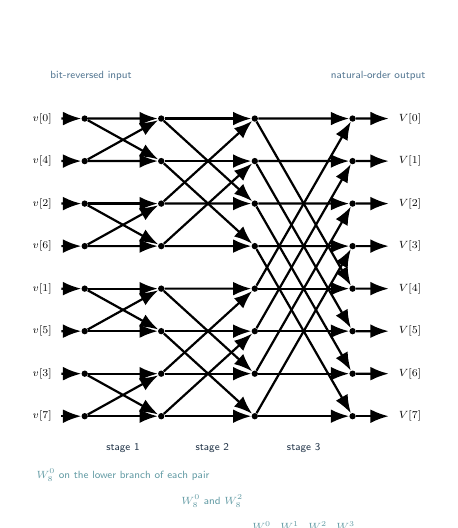
\begin{tikzpicture}[>=Latex, scale=0.54, transform shape, every node/.style={font=\scriptsize}]
    \foreach \y/\lin/\rout in {
      7/{\(v[0]\)}/{\(V[0]\)},
      6/{\(v[4]\)}/{\(V[1]\)},
      5/{\(v[2]\)}/{\(V[2]\)},
      4/{\(v[6]\)}/{\(V[3]\)},
      3/{\(v[1]\)}/{\(V[4]\)},
      2/{\(v[5]\)}/{\(V[5]\)},
      1/{\(v[3]\)}/{\(V[6]\)},
      0/{\(v[7]\)}/{\(V[7]\)}
    }{
      \node at (0,\y) {\lin};
      \node[fftdot] (szero\y) at (1.0,\y) {};
      \node[fftdot] (sone\y) at (2.8,\y) {};
      \node[fftdot] (stwo\y) at (5.0,\y) {};
      \node[fftdot] (sthree\y) at (7.3,\y) {};
      \node at (8.65,\y) {\rout};
      \draw[->, thick] (0.45,\y)--(szero\y);
      \draw[->, thick] (sthree\y)--(8.15,\y);
    }
    \foreach \a/\b in {7/6,5/4,3/2,1/0} {
      \draw[->, thick] (szero\a)--(sone\a);
      \draw[->, thick] (szero\b)--(sone\b);
      \draw[->, thick] (szero\a)--(sone\b);
      \draw[->, thick] (szero\b)--(sone\a);
    }
    \foreach \a/\b/\c/\d in {7/6/5/4,3/2/1/0} {
      \draw[->, thick] (sone\a)--(stwo\a);
      \draw[->, thick] (sone\b)--(stwo\b);
      \draw[->, thick] (sone\c)--(stwo\c);
      \draw[->, thick] (sone\d)--(stwo\d);
      \draw[->, thick] (sone\a)--(stwo\c);
      \draw[->, thick] (sone\c)--(stwo\a);
      \draw[->, thick] (sone\b)--(stwo\d);
      \draw[->, thick] (sone\d)--(stwo\b);
    }
    \foreach \a/\b in {7/3,6/2,5/1,4/0} {
      \draw[->, thick] (stwo\a)--(sthree\a);
      \draw[->, thick] (stwo\b)--(sthree\b);
      \draw[->, thick] (stwo\a)--(sthree\b);
      \draw[->, thick] (stwo\b)--(sthree\a);
    }
    \node[SecondaryColor] at (1.15,8.0) {bit-reversed input};
    \node[SecondaryColor] at (7.9,8.0) {natural-order output};
    \node[PrimaryColor] at (1.9,-0.75) {stage 1};
    \node[PrimaryColor] at (4.0,-0.75) {stage 2};
    \node[PrimaryColor] at (6.15,-0.75) {stage 3};
    \node[AccentColor] at (1.9,-1.38) {\(W_8^0\) on the lower branch of each pair};
    \node[AccentColor] at (4.0,-2.0) {\(W_8^0\) and \(W_8^2\)};
    \node[AccentColor] at (6.15,-2.62) {\(W_8^0,\ W_8^1,\ W_8^2,\ W_8^3\)};
  \end{tikzpicture}%
}

\begin{document}

\begin{center}
  {\LARGE \textbf{CSE 219 Practice Questions}}\\[0.24em]
  {\large FFT, Sampling, Laplace Transform, and z-Transform}
\end{center}

\tableofcontents
\newpage

\section{Radix-2 DIT Cooley-Tukey FFT}

\QuestionItem{Problem 1.1}{Starting from \(X[k]=\sum_{n=0}^{N-1}x[n]W_N^{kn}\), derive the radix-2 DIT split into even and odd subsequences and the butterfly relations for \(0\le k<N/2\).}

\QuestionItem{Problem 1.2}{Compute the 4-point DIT FFT of \(x[n]=[2,1,-3,4]\) using radix-2 butterflies.}

\QuestionItem{Problem 1.3}{Compute the 4-point DIT FFT of \(x[n]=[1,2,3,4]\) using radix-2 butterflies.}

\QuestionItem{Problem 1.4}{Compute the 8-point DIT FFT of \(x[n]=[1,2,0,-1,3,0,2,1]\) using the full radix-2 butterfly.}

\QuestionItem{Problem 1.5}{Recover \(x[n]\) from
  \[
    X[k]=[\,6,\ \sqrt2-j\sqrt2,\ 2+4j,\ -\sqrt2-j\sqrt2,\ -2,\ -\sqrt2+j\sqrt2,\ 2-4j,\ \sqrt2+j\sqrt2\,]
  \]
using an 8-point inverse FFT.}

\section{2D Matrix Formulation of Cooley-Tukey (Bailey's FFT)}

\QuestionItem{Problem 2.1}{Show how a 4-point DFT can be written as a \(2\times 2\) matrix factorization using column-major input, row DFTs, twiddles, and column DFTs.}

\QuestionItem{Problem 2.2}{Use a \(2\times 4\) Bailey factorization to compute the 8-point DFT of \(x[n]=[1,3,-1,2,0,4,2,1]\).}

\QuestionItem{Problem 2.4}{A 16-point sequence is \(x[n]=[1,0,0,0,\,2,0,0,0,\,-1,0,0,0,\,3,0,0,0]\). Use the \(4\times 4\) formulation to reduce the work.}

\section{Bluestein's FFT}

\QuestionItem{Problem 3.1}{Derive Bluestein's chirp identity
  \[
    W_N^{nk}=W_{2N}^{-(k-n)^2}W_{2N}^{k^2}W_{2N}^{n^2}.
\]}

\QuestionItem{Problem 3.2}{Use Bluestein's construction to compute the 3-point DFT of \(x[n]=[2,-1,3]\).}

\QuestionItem{Problem 3.3}{Run the same method on the 4-point sequence \(x[n]=[1,2,0,0]\) and compare with the ordinary 4-point DFT.}

\section{Application of FFT: Fast Convolution}

\QuestionItem{Problem 4.1}{Compute the linear convolution of \(x[n]=[1,2]\) and \(h[n]=[1,-1]\) using a 4-point FFT.}

\QuestionItem{Problem 4.2}{Compute the linear convolution of \(x[n]=[1,-1,2]\) and \(h[n]=[2,1]\) using a 4-point radix-2 FFT.}

\QuestionItem{Problem 4.3}{Compute the linear convolution of \(x[n]=[1,0,1]\) and \(h[n]=[1,-1,2]\). Use the smallest radix-2 FFT size.}

\QuestionItem{Problem 4.4}{Repeat Problem 4.3 incorrectly with a 4-point FFT and show the circular-convolution wrap-around.}

\section{Nyquist-Shannon Sampling Theorem}

\QuestionItem{Problem 5.1}{State the Nyquist-Shannon sampling theorem in both angular-frequency and ordinary-frequency form.}

\QuestionItem{Problem 5.2}{Derive the condition \(\omega_s>2\omega_M\) by comparing adjacent spectral copies of a bandlimited spectrum.}

\QuestionItem{Problem 5.3}{A lowpass signal is bandlimited to \(|f|\le 1.6\) kHz. Sketch the sampled spectrum for \(f_s=4.5\) kHz and for \(f_s=2.8\) kHz, and identify which case aliases.}

\QuestionItem{Problem 5.4}{A signal contains tones at \(1.2\) kHz and \(1.8\) kHz. Give one safe sampling frequency and one unsafe sampling frequency.}

\section{Ideal Reconstruction, Zero-Order Hold, Linear Interpolation}

\QuestionItem{Problem 6.1}{Write the impulse response and frequency response of the ideal reconstruction filter, and decide whether it is causal.}

\QuestionItem{Problem 6.2}{Derive the impulse response and frequency response of the zero-order hold (ZOH).}

\QuestionItem{Problem 6.3}{Derive the impulse response and frequency response of linear interpolation.}

\QuestionItem{Problem 6.4}{Compare the magnitude responses of ideal, ZOH, and linear interpolation at \(\omega=\omega_s/4\).}

\QuestionItem{Problem 6.5}{State one main advantage and one main drawback of each of the three reconstruction methods.}

\section{Laplace Transform: Definition, Properties, ROC, Poles and Zeros}

\QuestionItem{Problem 7.1}{Find the Laplace transform and ROC of \(x(t)=(t-2)e^{-3(t-2)}u(t-2)\).}

\QuestionItem{Problem 7.2}{Find the Laplace transform and ROC of \(x(t)=t^2 e^{-3t}u(t)\).}

\QuestionItem{Problem 7.3}{Find the Laplace transform and ROC of \(x(t)=t e^{-t}u(t)+e^{2t}u(-t)\).}

\QuestionItem{Problem 7.4}{Find the Laplace transform and ROC of \(x(t)=e^{-4(t-1)}\cos\!\bigl(3(t-1)\bigr)u(t-1)\).}

\QuestionItem{Problem 7.5}{Find the Laplace transform, ROC, poles, and zeros of \(x(t)=t e^{-t}\sin(2t)u(t)\).}

\QuestionItem{Problem 7.6}{Find the Laplace transform and ROC of \(y(t)=\bigl(e^{-t}\sin(3t)\,u(t)\bigr)*\bigl(e^{-2t}u(t)\bigr)\).}

\section{Inverse Laplace Transform}

\QuestionItem{Problem 8.1}{Invert \(X(s)=\dfrac{3s+7}{(s+1)(s+2)}\) with ROC \(\text{Re}\{s\}>-1\).}

\QuestionItem{Problem 8.2}{Invert \(X(s)=\dfrac{2s+3}{s^2+2s+5}\) with ROC \(\text{Re}\{s\}>-1\).}

\QuestionItem{Problem 8.3}{Invert \(X(s)=\dfrac{-5}{(s+1)(s-4)}\) with ROC \(-1<\text{Re}\{s\}<4\).}

\QuestionItem{Problem 8.4}{Invert \(X(s)=\dfrac{s}{(s^2+4)^2}\) with ROC \(\text{Re}\{s\}>0\).}

\QuestionItem{Problem 8.5}{Invert \(X(s)=\dfrac{e^{-s}}{s(s+2)}\) with ROC \(\text{Re}\{s\}>0\).}

\QuestionItem{Problem 8.6}{Invert \(X(s)=\dfrac{2}{s(s^2+4)}\) with ROC \(\text{Re}\{s\}>0\).}

\QuestionItem{Problem 8.7}{Invert \(X(s)=\dfrac{s}{s+2}\) with ROC \(\text{Re}\{s\}>-2\).}

\section{Applications of Laplace Transform}

\QuestionItem{Problem 9.1}{For \(H(s)=\dfrac{s+2}{(s+1)(s+2)}\), determine the admissible ROC choices and the corresponding causality/stability properties.}

\QuestionItem{Problem 9.2}{For \(H(s)=\dfrac{1}{(s+1)^2(s+3)}\), determine the admissible ROC choices and the corresponding causality/stability properties.}

\QuestionItem{Problem 9.3}{Decide whether the Fourier transform exists for \(X(s)=\dfrac{1-e^{-3(s+2)}}{s+2}\). Interpret the result in time domain.}

\QuestionItem{Problem 9.4}{Solve \(y'(t)+y(t)=e^{-2(t-1)}u(t-1)\) with \(y(0^-)=0\).}

\QuestionItem{Problem 9.5}{Solve \(y''(t)+3y'(t)+2y(t)=e^{-(t-1)}u(t-1)\) with zero initial conditions.}

\QuestionItem{Problem 9.6}{A causal LTI system is described by the LCCDE \(\dfrac{d^2 y}{dt^2}+5\dfrac{dy}{dt}+6y(t)=\dfrac{dx}{dt}+3x(t)\). Find \(H(s)\), sketch the pole--zero plot, determine whether the system is stable, and find the impulse response \(h(t)\).}

\section{z-Transform: Definition, Properties, ROC, Poles and Zeros}

\QuestionItem{Problem 10.1}{Find the z-transform, poles, zeros, and ROC of \(x[n]=\left(\frac34\right)^n\cos\!\left(\frac{\pi n}{3}\right)u[n]\).}

\QuestionItem{Problem 10.2}{Find the z-transform and ROC of \(x[n]=(n-2)\left(\frac13\right)^{n-2}u[n-2]\).}

\QuestionItem{Problem 10.3}{Find the z-transform, poles, zeros, and ROC of \(x[n]=\left(\frac14\right)^n u[n]-2^n u[-n-1]\).}

\QuestionItem{Problem 10.4}{Find the z-transform and zero pattern of \(x[n]=\delta[n]-2\delta[n-1]+2\delta[n-2]-\delta[n-3]\).}

\QuestionItem{Problem 10.5}{Find the z-transform, poles, zeros, and ROC of \(x[n]=\left(\frac12\right)^{n-1}\cos\!\left(\frac{\pi(n-1)}{3}\right)u[n-1]\).}

\QuestionItem{Problem 10.6}{Find the z-transform, poles, zeros, and ROC of \(y[n]=\bigl(\left(\frac12\right)^n u[n]\bigr)*\bigl(\left(\frac13\right)^n u[n]\bigr)\).}

\QuestionItem{Problem 10.7}{Let \(x[n]=\left(\frac12\right)^n u[n]\). Find the z-transform and ROC of the running sum \(y[n]=\displaystyle\sum_{k=-\infty}^{n}x[k]\).}

\section{Inverse z-Transform}

\QuestionItem{Problem 11.1}{Invert \(X(z)=\dfrac{2-z^{-1}}{(1-\frac14 z^{-1})(1-\frac34 z^{-1})}\) for \(|z|>\frac34\).}

\QuestionItem{Problem 11.2}{Invert \(X(z)=\dfrac{1}{(1-2z^{-1})(1-\frac13 z^{-1})}\) for \(\frac13<|z|<2\).}

\QuestionItem{Problem 11.3}{Invert \(X(z)=\dfrac{1-\frac56 z^{-1}}{(1-\frac12 z^{-1})(1-\frac13 z^{-1})}\) for \(|z|<\frac13\).}

\QuestionItem{Problem 11.4}{Invert \(X(z)=\dfrac{1+\frac12 z^{-1}}{\left(1-\frac12 z^{-1}\right)^2}\) for \(|z|>\frac12\).}

\QuestionItem{Problem 11.5}{Invert \(X(z)=z^{-1}\dfrac{1-\frac14 z^{-1}}{1-\frac12 z^{-1}+\frac14 z^{-2}}\) for \(|z|>\frac12\).}

\section{Applications of z-Transform: Causality, Stability from ROC}

\QuestionItem{Problem 12.1}{For \(H(z)=\dfrac{1-2z^{-1}}{(1-\frac12 z^{-1})(1-2z^{-1})}\), determine the valid ROC choices and the corresponding causality/stability/DTFT conclusions.}

\QuestionItem{Problem 12.2}{For \(H(z)=\dfrac{1}{(1-0.8 z^{-1})(1-1.25 z^{-1})}\), determine whether any realization can be both stable and causal.}

\QuestionItem{Problem 12.3}{Determine whether the DTFT exists for \(x[n]=\left(\frac12\right)^n u[n]-1.2^n u[-n-1]\).}

\QuestionItem{Problem 12.4}{Given \(h[n]=\left(\frac23\right)^n u[n]-\left(\frac43\right)^n u[-n-1]\), find \(H(z)\) and its ROC, and determine whether the system is causal, stable, and whether the DTFT of \(h[n]\) exists.}

\QuestionItem{Problem 12.5}{A system has poles at \(0.95e^{\pm j\pi/4}\) and \(1.1\). Determine whether there exists a stable realization, a causal realization, and a realization that is both.}

\end{document}
